\subsection{Virtual heart and pacemaker models}
\label{heartmodel}

The coordinated contractions of the heart muscles are governed by the generation and conduction of electrical signals throughout the heart. Anomalies in the timing and pattern of the electrical signals results in abnormal heart rhythms, or \emph{arrhythmia}. Implantable pacemakers are designed to treat a subset of arrhythmia by monitoring local electrical activities in the atria and the ventricles and deliver electrical pacing to maintain appropriate heart rhythm. %Since we don't have access to real human hearts for testing, we have developed a \emph{Virtual Heart Model (VHM)}, which simulates the \emph{timing aspects} of the operation of a human heart, and ignores other physiological details.
%\todo[inline]{ZJ : review following for accuracy}

The electrical activity of the heart is studied extensively in \emph{Electrophysiology} (EP)~\cite{josephson}. 
The EP principles describe the majority of heart conditions, and are the foundation of all pacemaker operations. 
In \cite{VHM_proc} we developed the Virtual Heart Model (VHM) based on the EP principles. 
The VHM uses Finite State Machines (FSM) to model anatomical and/or topological structures of the electrical conduction system of the heart. 
The refractory properties of heart tissue are captured using node FSMs and the conduction delays between nodes are captured by the path FSMs. 
See Fig.~\ref{fig:FSMSA} for an example of a node FSM. 
By assembling node and path FSMs with different parameters we are able to simulate different heart conditions, and more importantly, their interaction with any pacemakers.
\begin{figure}[t]
\centering
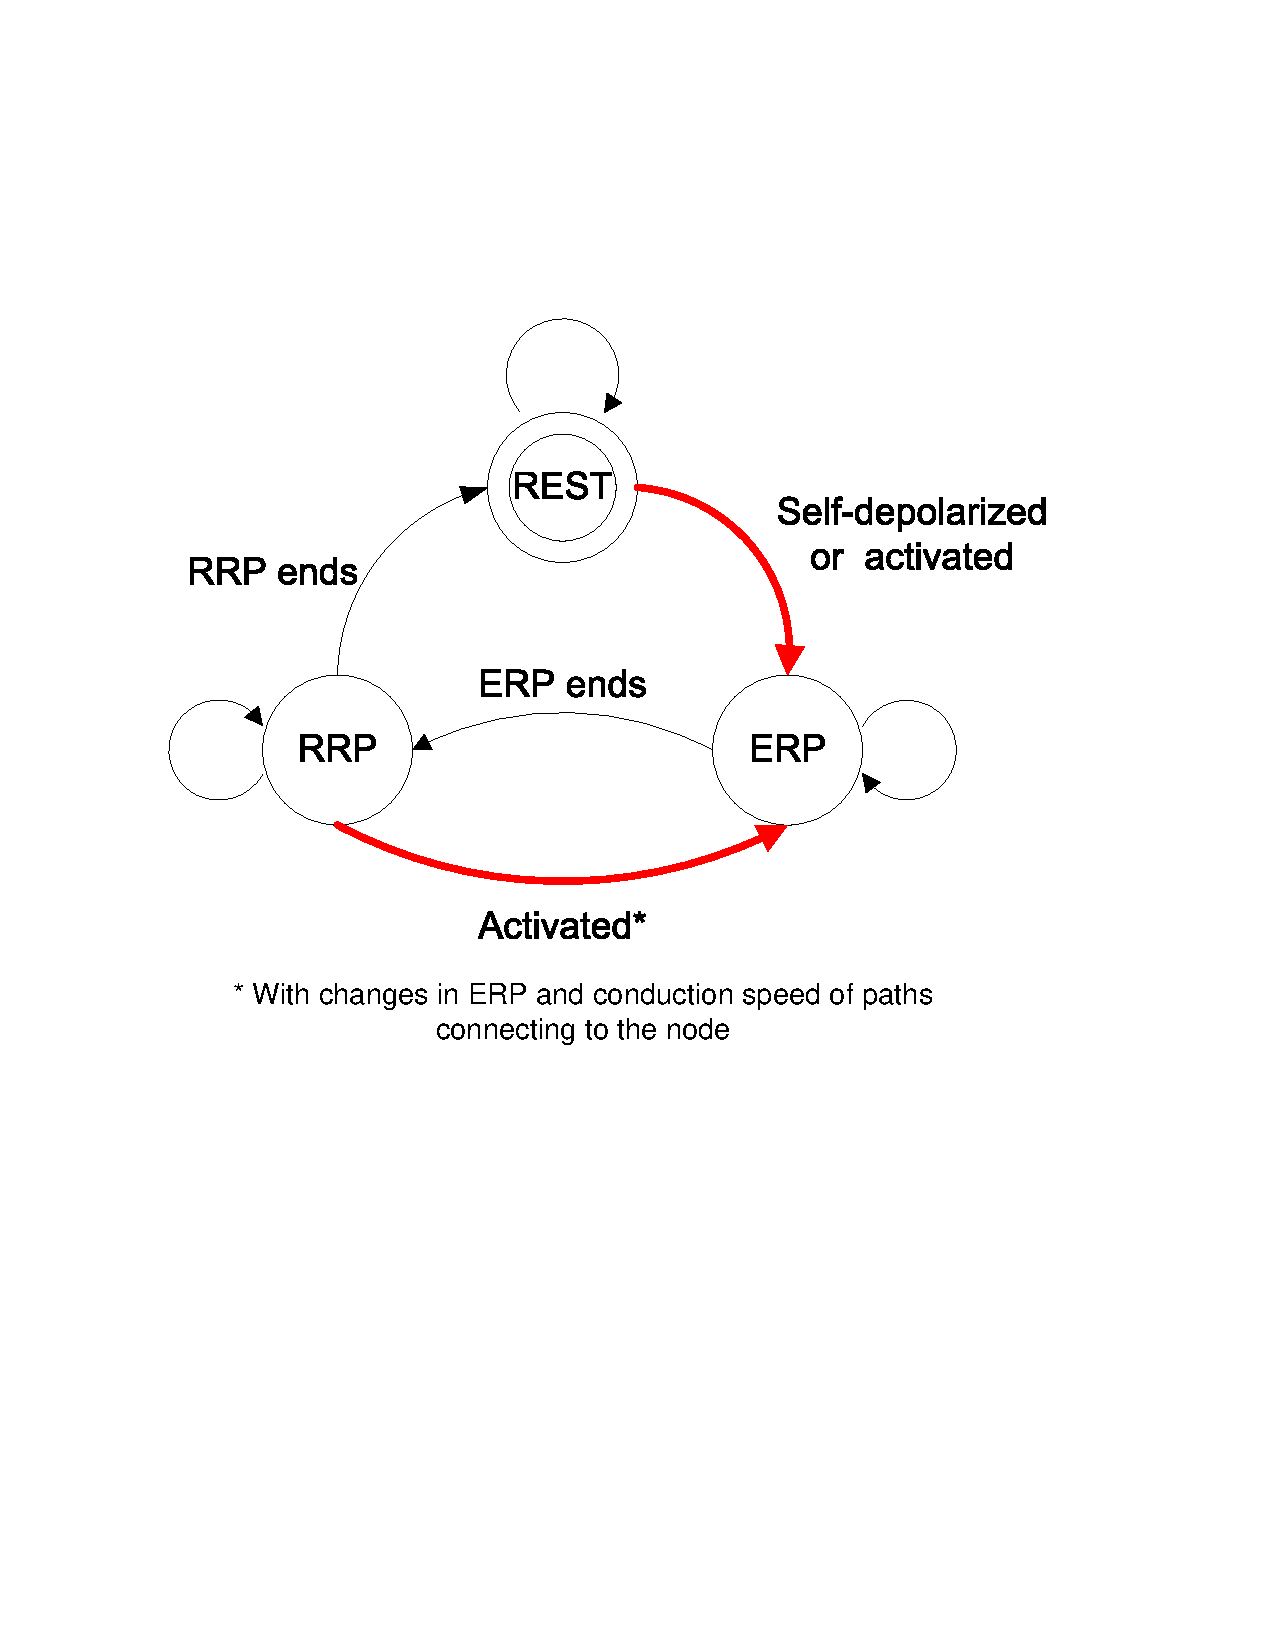
\includegraphics[scale=0.4]{node_automata.pdf}
\caption{FSM modeling the SA node showing Effective and Relative Refractory Periods (ERP and RRP) and the Rest state.}
\label{fig:FSMSA}
\vspace{-.5cm}
\end{figure}
%The VHM is implemented in both Simulink and Matlab. 
%We used the VHM to simulate different heart conditions in a closed loop with the pacemaker model, such as Wenckebach AV nodal response, atrial flutter and pacemaker mediated tachycardia.
The VHM functional output has been validated by the director of cardiac electrophysiology in the Philadelphia VA Hospital and by electrophysiologists in the Hospital of the University of Pennsylvania. 
More details are available in \cite{VHM_proc}.

To run the experiments in this paper, we used a DDD pacemaker model developed according to the specification derived from the Boston Scientific Challenge~\cite{challenge}.
%\todo[inline]{ZJ : 2-3 lines describing the PM model.}
The model has been validated against the specifications using open-loop testing \cite{testing}. 
Local electrical impulses in the atrium and the ventricle can trigger $AS$ and $VS$ events, respectively. The pacemaker can deliver electrical pacing from the atrial lead ($AP$) and the ventricular lead ($VP$). 
The most basic function of a DDD pacemaker is described as follows: 
from any ventricular events (VS,VP), if no AS appear within $TLRI-TAVI$, the pacemaker will deliver AP. 
From any atrial events (AS,AP), if no VS appear within $TAVI$ and the interval from the last ventricular event (VS,VP) is longer than $TURI$, the  pacemaker will deliver VP. 
Together these two functions guarantee that the ventricular rate of the heart maintained above $60000/TLRI$ beats per minute (bpm) and the paced ventricular rate is lower than $60000/TURI$ bpm.
%More information about the implementation can be found in \cite{testing}. 

%\textbf{1. Lower Rate Interval (LRI)}:
%The LRI interval starts at a ventricular sensed or paced event. The LRI interval is the longest interval between two ventricular events. 
%
%\textbf{2. Upper Rate Interval (URI)}:
%The URI interval defines the shortest interval between a ventricular event and a paced ventricular event
%
%\textbf{3. Atrial-Ventricular Interval (AVI)}:
%Ventricular pacing shall occur in the absence of a sensed ventricular event within the programmed AV delay when the time elapsed after the last ventricular event is between the programmed LRI and URI.
%
%\textbf{4. Ventricular Refractory Period (VRP)}:
%The VRP is the time interval following a ventricular event during which no ventricular sense (VS) can happen.
%
%\textbf{5. Post Ventricular Atrial Refractory Period (PVARP)}:
%The PVARP is the time interval following a ventricular event during which no atrial sense (AS) can happen.
%
%According to the five primary specifications of the basic DDD pacemaker, a Simulink model was designed using temporal logic. Each component corresponds to a particular specification and communicates with others using channels. A timing diagram is shown in \ref{timingPM}. 
%%%%%%%%%%%%%%%%%%%%%%%%%%%%%%%%%%%%%%%%%%%%%%%
%\begin{figure}[!b]
%	\center
%	\vspace{-10pt}
%	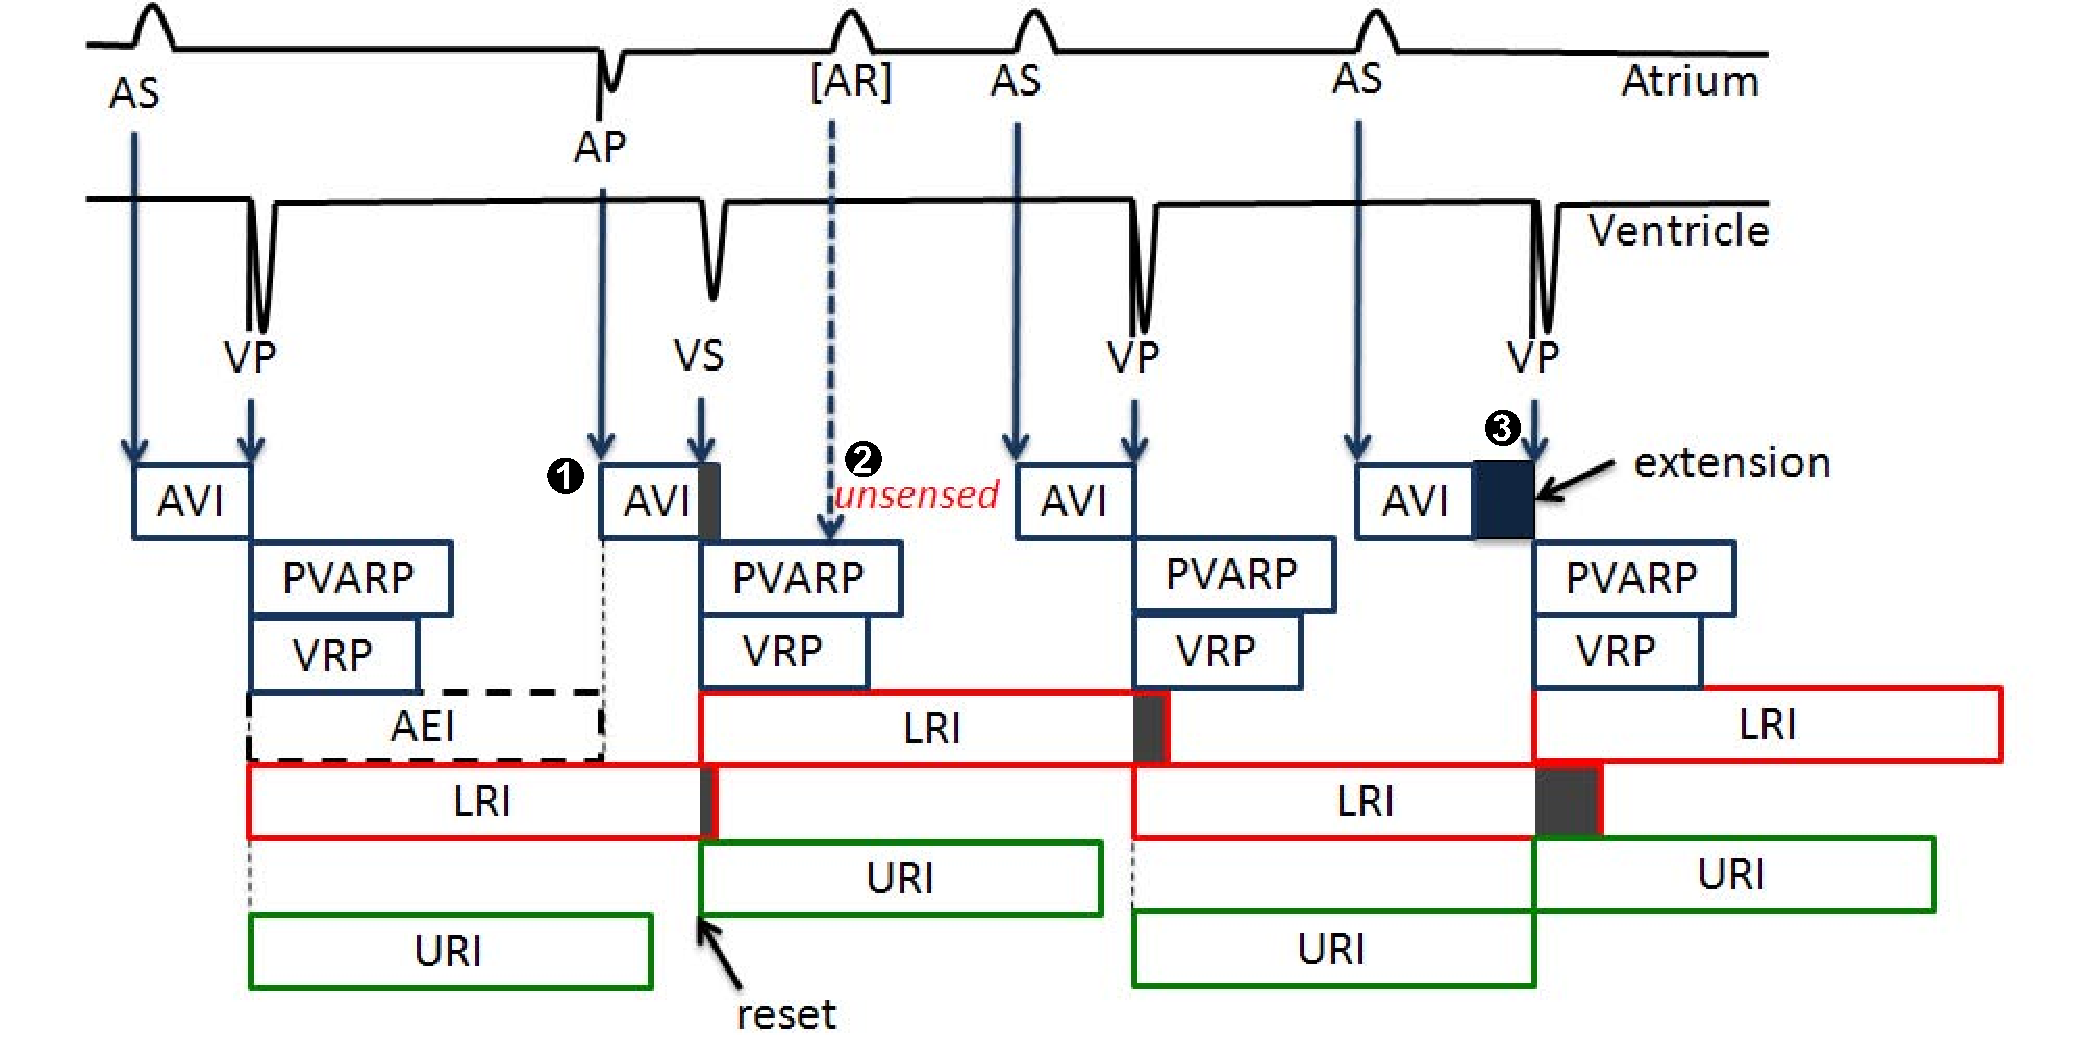
\includegraphics[width=0.45\textwidth]{figures/PM_timers.pdf}
%	\vspace{-10pt}
%	\caption{Simulink design of path automata}
%	\label{fig:timingPM}
%\end{figure}